Au sein du FabLab, on appelle outil numérique les machines qui sont pilotées par un ordinateur. Les deux machines les plus spectaculaires : l'imprimante 3D et la découpeuse laser. Elles sont reliées par l'intermédiaire d'un simple câble à l'ordinateur destiné à leur faire parvenir les travaux à effectuer.

\begin{center}
L'utilisation des ces deux appareils est soumise à une formation et à la présence d'un référent.
\end{center}
\subsection{L'imprimante 3D}
\begin{wrapfigure}{r}{45mm}
\centering
    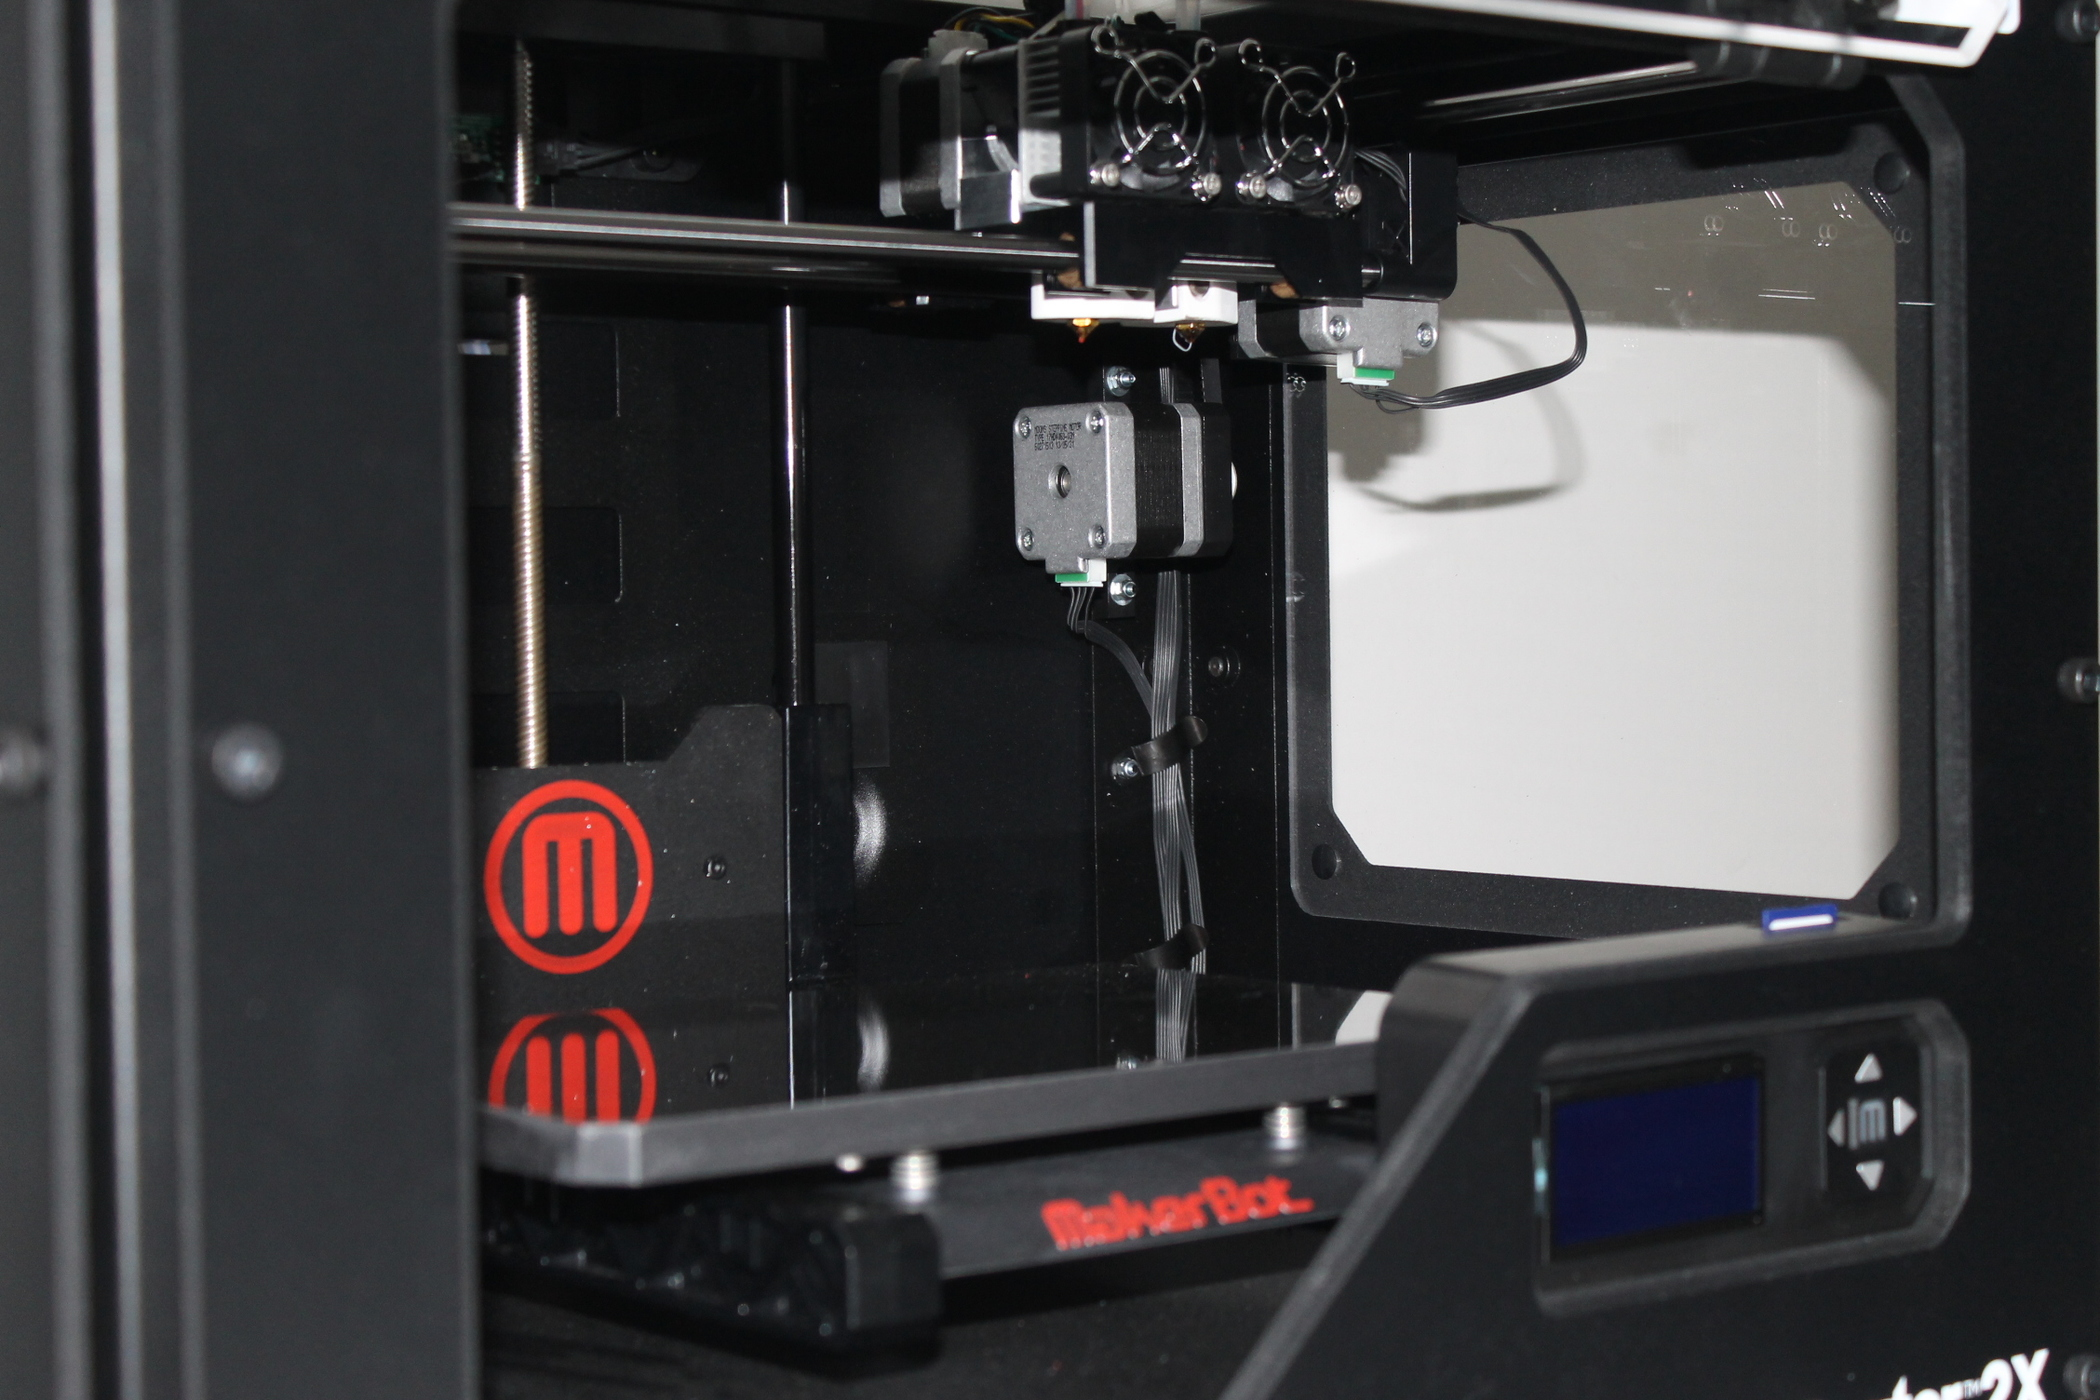
\includegraphics[width=40mm]{Makerbot2X.jpg}
%    \caption{Makerbot Replicator 2X (vue intérieure)}
    \label{fig:imprimante3D}
\end{wrapfigure}

Par rapport à une imprimante classique qui imprime en 2D, l'imprimante 3D ajoute la notion de hauteur. En empilant des couches successives de plastique, il est alors possible de fabriquer des objets en volume tels qu'ils ont été conçus dans un logiciel de modélisation.
Le FabLab de Pau possède une \textit{Makerbot Replicator 2X}.

\begin{itemize}
  \item Surface utile du plateau : 246 mm $\times$ 152mm
  \item Hauteur maximale de l'objet imprimé : 155 mm
  \item Matériau utilisé : ABS en filament de 1,75 mm de diamètre
  \item Diamètre de la tête : 0,4 mm
  \item Épaisseur des couches : 0,1 mm
\end{itemize}

\subsection{Graveuse/découpeuse Laser}
\begin{wrapfigure}{l}{45mm}
\centering
    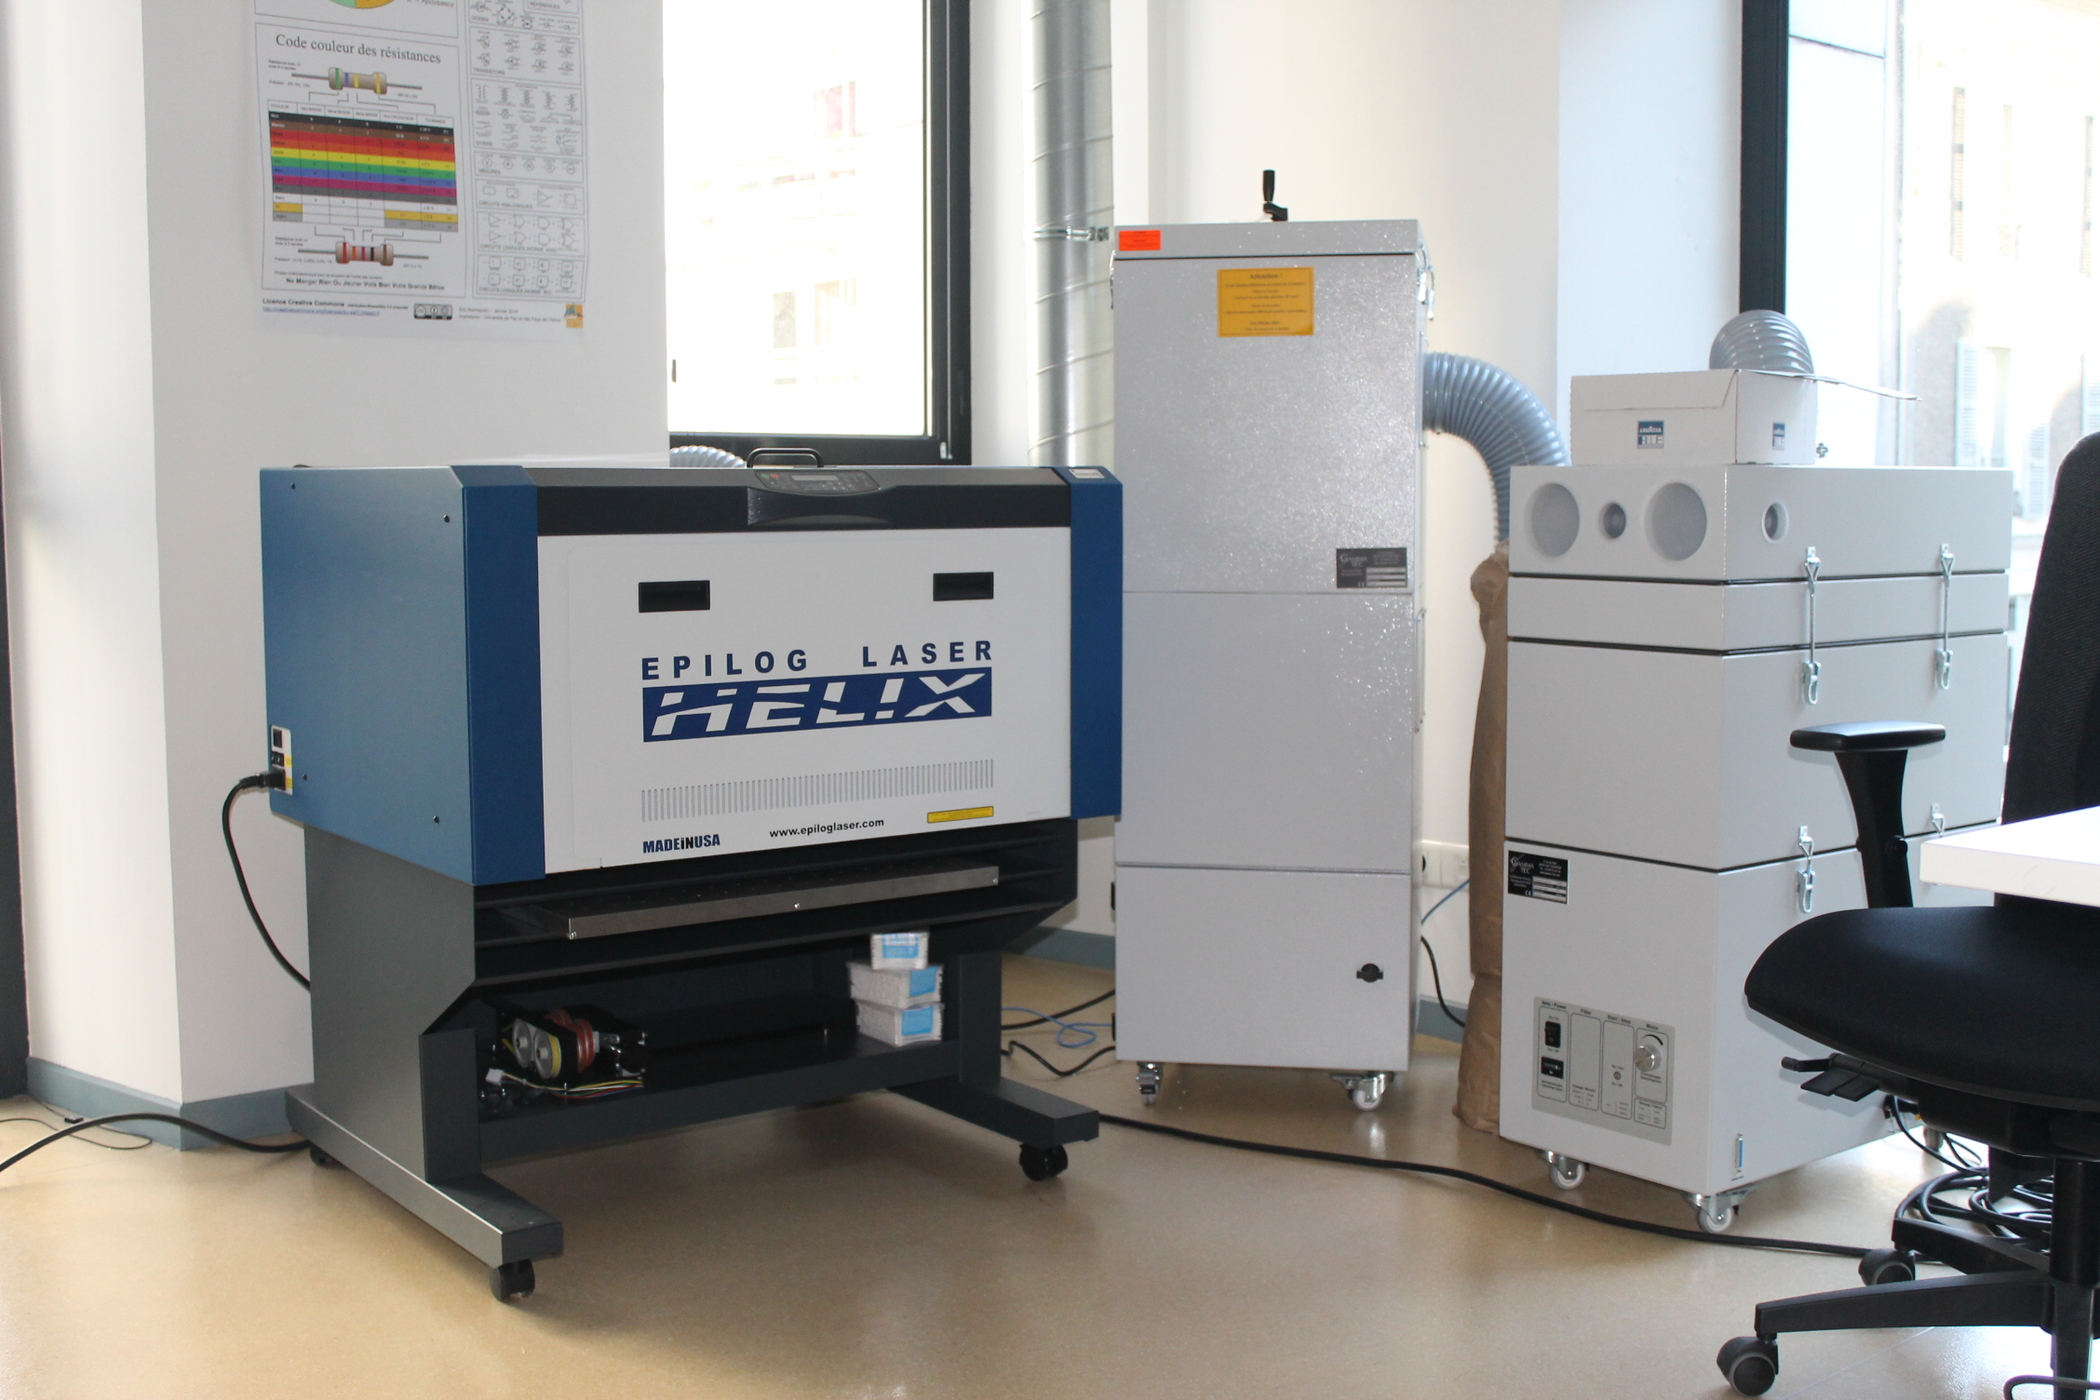
\includegraphics[width=40mm]{Epilog.jpg}
%    \caption{Epilog Helix}
    \label{fig:decoupeuselaser}
\end{wrapfigure}
Après avoir fait une rapide mise au point, un laser très puissant se déplace sur la surface du matériau placé sur la zone de travail. En fonction de la puissance pour laquelle il est programmé, ce laser va graver ou découper. La diversité des matériaux utilisables, la finesse et la précision du faisceau permettent d'obtenir très rapidement des résultats bluffants.
Le FabLab de Pau possède une \textit{Épilog Hélix 75W}.

\begin{itemize}
  \item Surface utile du plateau : 609 mm $\times$ 456 mm
  \item Hauteur maximale de l'objet gravé ou découpé : 229 mm
  \item Matériaux autorisés : papier, carton, bois, cuir, verre (gravure uniquement), plexiglas, \dots
  \item Matériaux strictement interdits : matières contenant du chlore (P.V.C., vinyle, skaï, \dots), porcelaine.
  \item Le laser ne peut pas découper le métal.
\end{itemize}

\subsection{Le petit outillage}
Le FabLab possède de nombreux petits outils comme des tournevis de précisions, une mini perçeuse \textit{Dremel}, des multimétres, une pince ampèremétrique, des fers à souder, un oscilloscope numérique, \dots

\subsection{Cartes programmables et mini-ordinateurs}
Utiles à de nombreux projets de domotiques ou autres projets embarqués, des cartes programmables de type \textit{Arduino} ou \textit{Grove} sont disponibles afin de prototyper son projet au FabLab. Si le projet nécessite une plus grande puissance de calcul, un accès réseau de type rapide Ethernet ou WiFi, ou encore une programmation complexe, des plateformes de développement \textit{Raspberry Pi} ou \textit{CubieBoard} sont disponibles.

\subsection{Le Cray}
Besoin d'encore plus de puissance de calcul ? Le FabLab possède un \textit{Cray}, c'est-à-dire un supercalculateur composé de 4 lames de calculs qu'il est possible d'agréger si besoin. Chaque lame possède 4 \textit{Intel Xéon} quadcore (soit 16 c\oe urs) cadencés à 3 Ghz, 32 GB de mémoire vive à correction d'erreurs, et 320 GB de disque-dur. Afin d'augmenter encore la capacités de calculs des processeur graphique \textit{nVidia Tesla} peuvent être exploités avec le langage de programmation CUDA\footnote{\url{http://www.nvidia.fr/object/cuda-parallel-computing-fr.html}}.
\begin{figure}[h]
  \begin{center}
    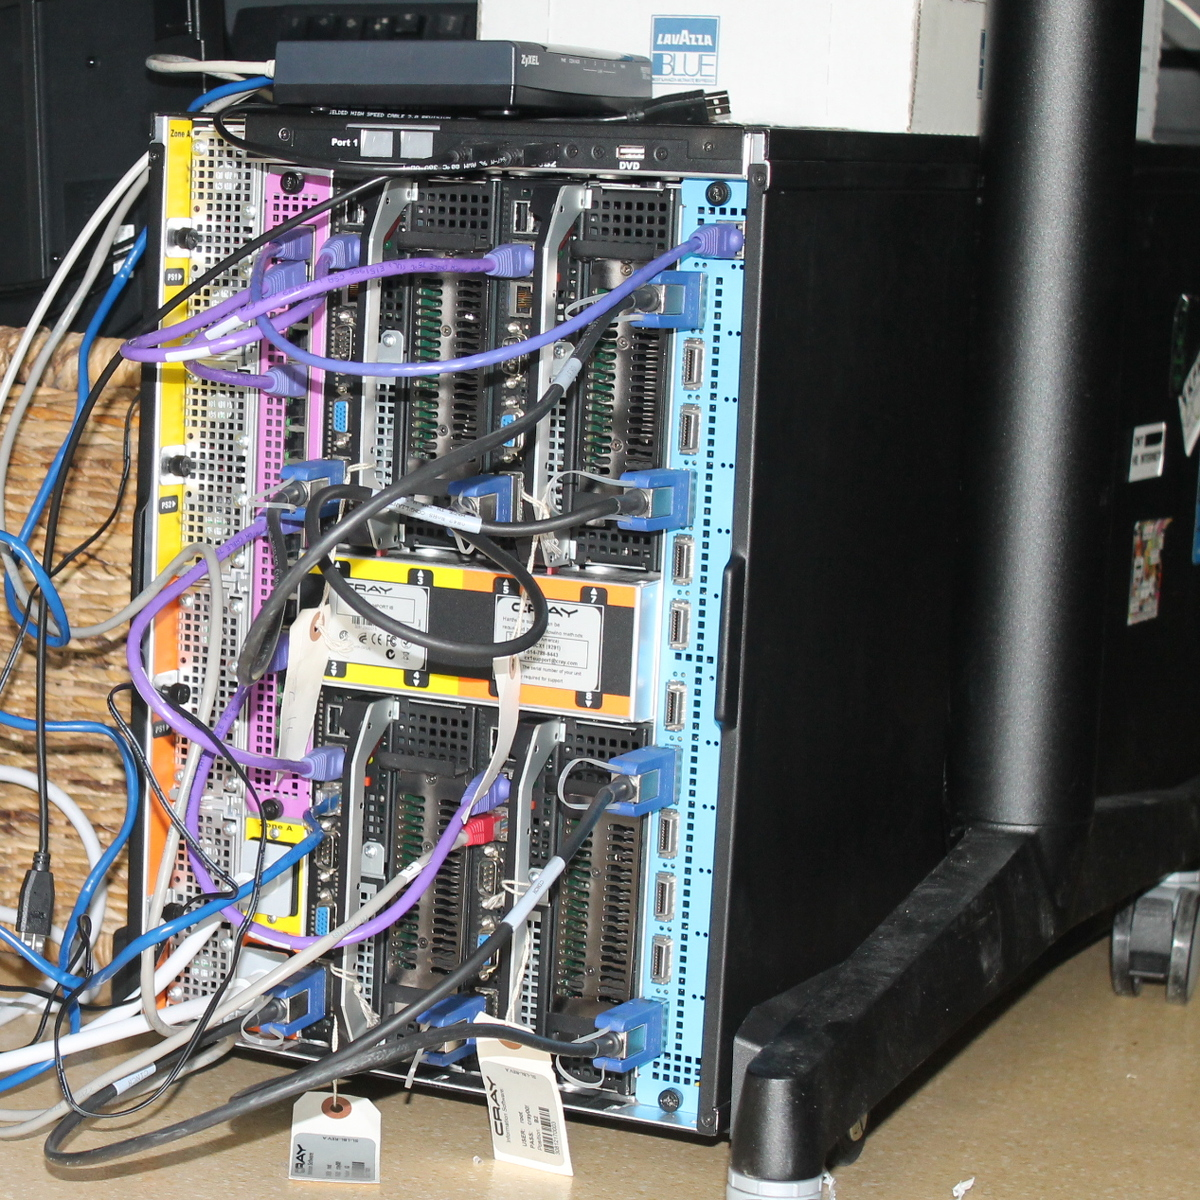
\includegraphics[height=75mm]{Cray.jpg}
%    \caption{}
    \label{fig:cray}
  \end{center}
\end{figure}
